\begin{figure} [h]
    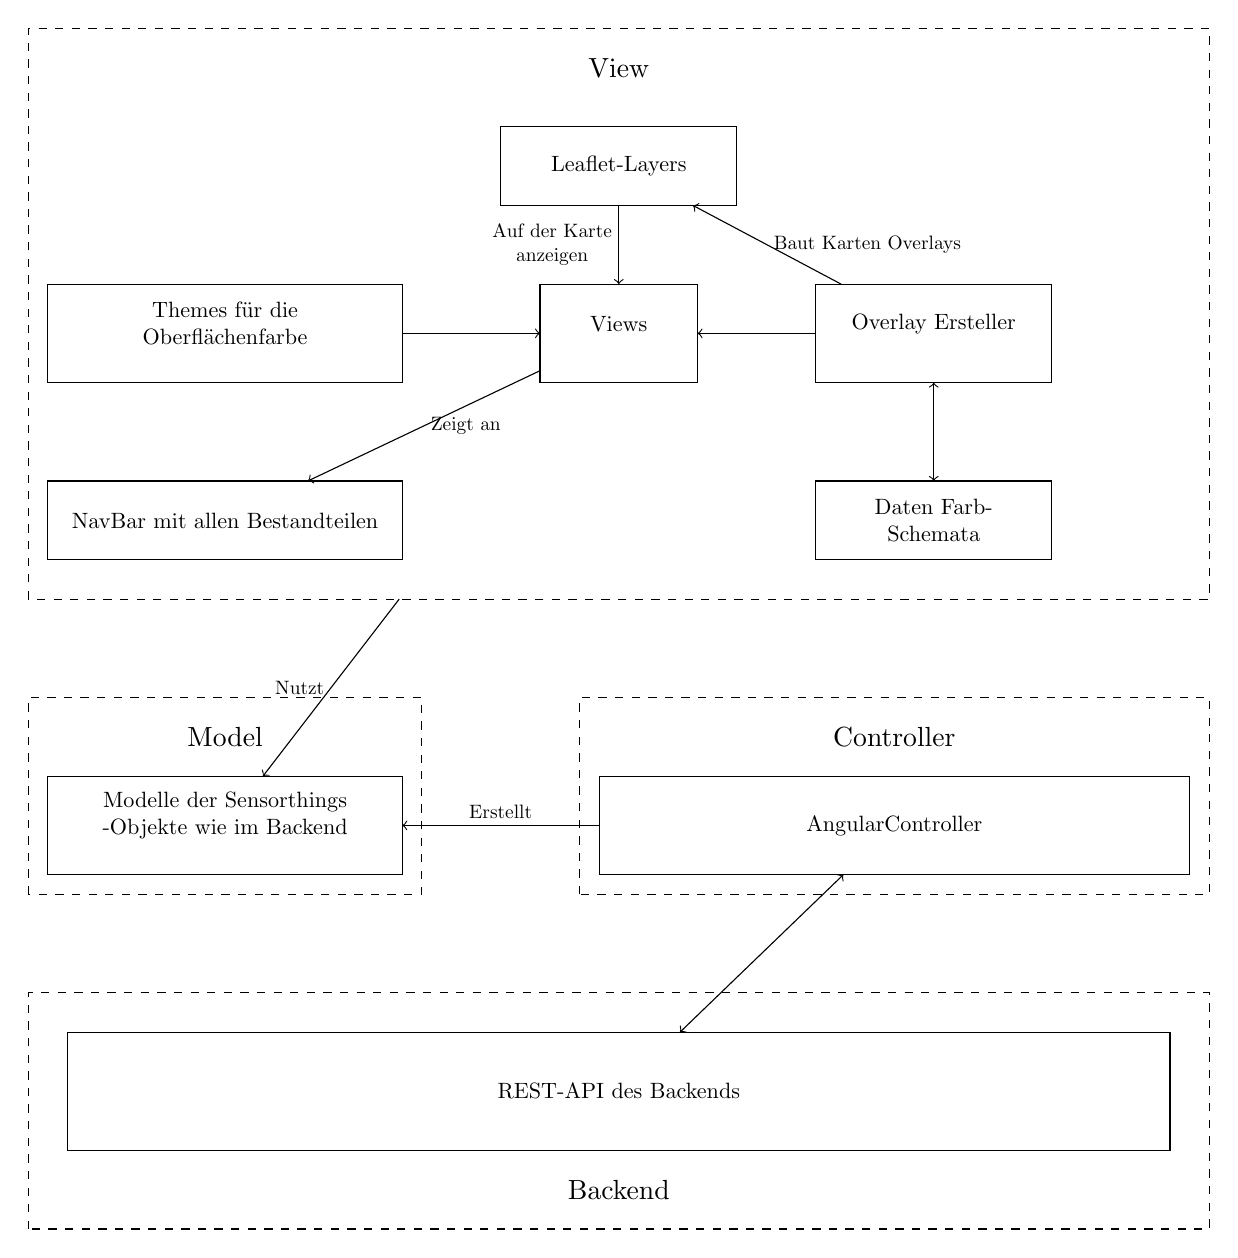
\begin{tikzpicture}[node distance=2cm]

        %View
        \begin{scope}[shift={(0,8)},local bounding box=View]
            \draw (0,0) [dashed] rectangle (15,7.25);
            \node[scale=1] at (7.5,6.75) {View};
            \begin{scope}[local bounding box=Themes]
                \draw (0.25,2.75) rectangle (4.75,4);
                \node[scale=0.8,align=center] at (2.5,3.5) {Themes für die\\Oberflächenfarbe};
            \end{scope}
            \begin{scope}[local bounding box=Views]
                \draw (6.5,2.75) rectangle (8.5,4);
                \node[scale=0.8,align=center] at (7.5,3.5) {Views};
            \end{scope}
            \begin{scope}[local bounding box=Leaflet]
                \draw (6,5) rectangle (9,6);
                \node[scale=0.8,align=center] at (7.5,5.5) {Leaflet-Layers};
            \end{scope}
            \begin{scope}[local bounding box=OverlayBuilder]
                \draw (10,2.75) rectangle (13,4);
                \node[scale=0.8,align=center] at (11.5,3.5) {Overlay Ersteller};
            \end{scope}
            \begin{scope}[local bounding box=NavBar]
                \draw (0.25,1.5) rectangle (4.75,.5);
                \node[scale=0.8,align=center] at (2.5,1) {NavBar mit allen Bestandteilen};
            \end{scope}
            \begin{scope}[local bounding box=aqd]
                \draw (10,1.5) rectangle (13,.5);
                \node[scale=0.8,align=center] at (11.5,1) {Daten Farb-\\Schemata};
            \end{scope}
        \end{scope}

        %Model
        \begin{scope}[shift={(0,4.25)},local bounding box=Model]
            \draw (0,0) [dashed] rectangle (5,2.5);
            \node[scale=1] at (2.5,2) {Model};
            \begin{scope}[local bounding box=STM]
                \draw (0.25,0.25) rectangle (4.75,1.5);
                \node[scale=0.8,align=center] at (2.5,1) {Modelle der Sensorthings\\-Objekte wie im Backend};
            \end{scope}
        \end{scope}
        
        %Controller
        \begin{scope}[shift={(7,4.25)},local bounding box=Controller]
            \draw (0,0) [dashed] rectangle (8,2.5);
            \node[scale=1] at (4,2) {Controller};
            \begin{scope}[local bounding box=ACon]
                \draw (0.25,0.25) rectangle (7.75,1.5);
                \node[scale=0.8, align=center] at (4,.875) {AngularController};
            \end{scope}
        \end{scope}

        %Backend
        \begin{scope}[shift={(0,0)},local bounding box=Backend]
            \draw (0,0) [dashed] rectangle (15,3);
            \node[scale=1] at (7.5,0.5) {\softwarename Backend};
            \begin{scope}[local bounding box=RESTAPI]
                \draw (0.5,1) rectangle (14.5,2.5);
                \node[scale=0.8, align=center] at (7.5,1.75) {REST-API des \softwarename Backends};
            \end{scope}
        \end{scope}

        \draw[->] (View) -- (STM) node[midway,left,scale=0.7,align=center] {Nutzt};
        \draw[->] (ACon.west) -- (STM.east) node[midway,above,scale=0.7,align=center] {Erstellt};
        \draw[<->] (ACon) -- (RESTAPI);
        \draw[->] (Leaflet) -- (Views) node[midway,left,scale=0.7,align=center] {Auf der Karte\\anzeigen};
        \draw[->] (Themes) -- (Views);
        \draw[->] (OverlayBuilder) -- (Views);
        \draw[->] (OverlayBuilder) -- (Leaflet) node[midway,right,scale=0.7,align=center] {Baut Karten Overlays};
        \draw[->] (Views) -- (NavBar) node[midway,right,scale=0.7,align=center] {Zeigt an};
        \draw[<->] (aqd) -- (OverlayBuilder);
    \end{tikzpicture}
    \caption{Aufbau des \softwarename Frontends}
\end{figure}